\documentclass{article}

\usepackage{amsmath}
\usepackage{amsthm}
\usepackage{amsfonts}
\usepackage{amssymb}
\usepackage{dtklogos}
\usepackage{fullpage}
\usepackage{hyperref}
\usepackage{listings}
\usepackage{tikz} 
\usepackage{verbatimbox}
\usepackage{xcolor}

%% TKIZ arrows
\usetikzlibrary{arrows}

\newcommand{\vers}{0.70}
\newcommand{\tomemail}{thomas.allen@uky.edu}

\DeclareMathOperator{\dom}{Dom}

\newcommand\copyrighttext{%
  \footnotesize Copyright \copyright{} 2015 Thomas E. Allen.
  Permission is granted to copy, distribute and/or modify this
  document under the terms of the GNU Free Documentation License,
  Version 1.3 or any later version published by the Free Software
  Foundation; with no Invariant Sections, no Front-Cover Texts, and no
  Back-Cover Texts.  A copy of the license is included in the section
  entitled ``GNU Free Documentation License.''}
\newcommand\copyrightnotice{%
\begin{tikzpicture}[remember picture,overlay]
\node[anchor=south,yshift=10pt] at (current page.south) {\fbox{\parbox{\dimexpr\textwidth-\fboxsep-\fboxrule\relax}{\copyrighttext}}};
\end{tikzpicture}%
}

\title{A Guide to the CP-net Generator}

\author{Thomas E.~Allen}
\date{Version \vers{} (December 2015)}
\begin{document}
\maketitle

\copyrightnotice

\section{Introduction}

The CP-net Generator (GenCPnet) generates acyclic conditional
preference networks (CP-nets)~\cite{boutilier2004cp} uniformly at
random with respect to a specified set.  It is possible to specify
parameters such as the number of nodes, bound on indegree, and the
size of domains.

GenCPnet implements the method described in our paper, ``Generating
CP-nets Uniformly at Random''~\cite{generating_cpnets}.  If you use or
adapt this software, we kindly ask that you would cite our paper.
GenCPnet is free software, released under the GNU Public License
version 3.
%%
GenCPNet is written in C++ and designed to run on a GNU Linux system.
Throughout this manual, we assume the reader has access to such a
system and is familiar with using the command line to perform simple
instructions.
%%
Please email questions or bug reports to
\href{mailto:\tomemail}{\tomemail}.

\section{Obtaining GenCPnet}

Presently the software and documentation is housed at
%%
\begin{center}
\url{http://cs.uky.edu/~goldsmit/papers/GeneratingCPnetCode.html}.  
\end{center}
%%
\noindent The code can be downloaded as a zipped archive via a link on
that page.  Alternatively, you can download the archive directly with:
\begin{center}
\texttt{wget }\url{http://cs.uky.edu/~goldsmit/papers/gencpnet_0.70.zip}
\end{center}
or
\begin{center}
\texttt{wget }\url{http://cs.uky.edu/~teal223/gencpnet_0.70.zip}
\end{center}

\section{Installing GenCPnet}

The GNU MultiPrecision (GMP) library must be installed to compile or
run GenCPnet.  If GMP is not present, you can install it with your
distribution's package manager.  For more information on GMP, see
\url{https://gmplib.org/}.

Once GMP is present, it should be straightforward to build GenCPnet on
a GNU Linux system:
%%
\begin{verbatim}
unzip gencpnet_0.70.zip
cd gencpnet_0.70
make
\end{verbatim}
%%
If the build is successful, the message \texttt{Success!}~will appear
on the last line of the output.  It should then be possible to run
GenCPNet directly within the build directory.  For example, try:
%%
\begin{verbatim}
./gencpnet --help
\end{verbatim}

You may also wish to copy the executable file \texttt{gencpnet} to a
suitable directory in your path.  For example,
%%
\begin{verbatim}
make install
\end{verbatim}
%%
copies the executable file to your \verb|~/bin| directory by default.
%%
If you wish to make the program available to all users on the system,
you can do so with a command such as:
%%
\begin{verbatim}
sudo cp gencpnet /usr/local/bin
\end{verbatim}
%%
You may need assistance from your system administrator with these
latter steps.  Finally, you may wish to edit \texttt{Makefile} itself.
The comments in the file provide additional installation and
customization details.

\section{Using the CP-net Generator}

Typing \texttt{./gencpnet --version} from within the
\verb|gencpnet_0.70| build directory shows the current version:
%%
\begin{verbatim}
$ ./gencpnet --version
CP-net Generator 0.70
Copyright (C) 2015 Thomas E. Allen
This is free software; see the source for copying conditions.
CP-net Generator comes with ABSOLUTELY NO WARRANTY.
\end{verbatim}
%%
If you are working in a different directory and the GenCPnet
executable file is installed to a directory in your path, you should
omit the \texttt{./} and simply type \texttt{gencpnet} in all of the 
examples in this guide.
\begin{verbatim}
$ gencpnet --version
\end{verbatim}
Note that the
\verb|$| in these examples is the command line prompt and should not
be typed.

\subsection{The \texttt{-n} parameter: a simple binary-valued example}

We begin with a couple of very simple examples.  First, we show how to
generate a single CP-net with 3 nodes and binary domains:
\begin{verbatim}
$ mkdir examples
$ ./gencpnet -n 3 examples
Building distribution tables for CP-nets with the following specs:
Number of nodes: n = 3
Bound on in-degree c = 2
Homogeneous domains of size d = 2
Probability of incompleteness i = 0
Generating 1 random CP-nets with these specs.
Generation complete.
\end{verbatim}

Executing GenCPnet with the \verb|-n| option specifies that the CP-net
thus generated should be sampled from CP-nets with $n=3$ nodes.  By
default, the CP-nets in the set have unbounded indegree (a node may
have 0, 1, or 2 parents), and the domains are binary.  In this case
the generated example is written in XML format to the \verb|examples|
directory:
%%
\begin{verbatim}
$ ls -l examples
total 4
-rw-rw-r-- 1 user user 1932 Dec 15 14:49 cpnet_n3c2d2_0000.xml
\end{verbatim}
%%
The \verb|cpnet_n3c2d2_0000.xml| filename describes the parameters of
the generated CP-net instance:
\begin{itemize}
\item \verb|n3| indicates that the CP-net has $n=3$ nodes;
\item \verb|c2| indicates that a node can at most $c=2$ parents;
\item \verb|d2| indicates that the domains are all of size $d=2$. 
\item \verb|_0000| is an index number.  If we had generated multiple
  CP-nets using the \verb|-g| option described below, then these would
  be numbered sequentially from 0000.
\end{itemize}

Note that if we attempt to perform the identical command a second
time, an error message would result:
\begin{verbatim}
Error: filename cpnet_n3c2d2_0000.xml already exists.
Delete file(s) first or output to another directory.
\end{verbatim}
By throwing the error message, we avoid the unfortunate possibility of
overwriting the sets that we have previously generated, since these
may be needed for later experiments or in case later researchers wish
to confirm our results using the same input.

The format of the XML file is described in detail at the site
\url{http://www.ece.iastate.edu/~gsanthan/crisner.html}.  Here we only
describe it briefly.  Note that since our algorithm is randomized, the
output will likely differ on each execution. 

\begin{verbnobox}[\tiny\arabic{VerbboxLineNo}\small\hspace{3ex}]
<PREFERENCE-SPECIFICATION>

<PREFERENCE-VARIABLE>
 <VARIABLE-NAME>x1</VARIABLE-NAME>
 <DOMAIN-VALUE>1</DOMAIN-VALUE>
 <DOMAIN-VALUE>2</DOMAIN-VALUE>
</PREFERENCE-VARIABLE>

<PREFERENCE-VARIABLE>
 <VARIABLE-NAME>x2</VARIABLE-NAME>
 <DOMAIN-VALUE>1</DOMAIN-VALUE>
 <DOMAIN-VALUE>2</DOMAIN-VALUE>
</PREFERENCE-VARIABLE>

<PREFERENCE-VARIABLE>
 <VARIABLE-NAME>x3</VARIABLE-NAME>
 <DOMAIN-VALUE>1</DOMAIN-VALUE>
 <DOMAIN-VALUE>2</DOMAIN-VALUE>
</PREFERENCE-VARIABLE>

<PREFERENCE-STATEMENT>
  <STATEMENT-ID>p1_1</STATEMENT-ID>
  <PREFERENCE-VARIABLE>x1</PREFERENCE-VARIABLE>
  <PREFERENCE>2:1</PREFERENCE>
</PREFERENCE-STATEMENT>

<PREFERENCE-STATEMENT>
  <STATEMENT-ID>p2_1</STATEMENT-ID>
  <PREFERENCE-VARIABLE>x2</PREFERENCE-VARIABLE>
  <CONDITION>x1=1</CONDITION>
  <CONDITION>x3=1</CONDITION>
  <PREFERENCE>1:2</PREFERENCE>
</PREFERENCE-STATEMENT>

<PREFERENCE-STATEMENT>
  <STATEMENT-ID>p2_2</STATEMENT-ID>
  <PREFERENCE-VARIABLE>x2</PREFERENCE-VARIABLE>
  <CONDITION>x1=1</CONDITION>
  <CONDITION>x3=2</CONDITION>
  <PREFERENCE>1:2</PREFERENCE>
</PREFERENCE-STATEMENT>

<PREFERENCE-STATEMENT>
  <STATEMENT-ID>p2_3</STATEMENT-ID>
  <PREFERENCE-VARIABLE>x2</PREFERENCE-VARIABLE>
  <CONDITION>x1=2</CONDITION>
  <CONDITION>x3=1</CONDITION>
  <PREFERENCE>2:1</PREFERENCE>
</PREFERENCE-STATEMENT>

<PREFERENCE-STATEMENT>
  <STATEMENT-ID>p2_4</STATEMENT-ID>
  <PREFERENCE-VARIABLE>x2</PREFERENCE-VARIABLE>
  <CONDITION>x1=2</CONDITION>
  <CONDITION>x3=2</CONDITION>
  <PREFERENCE>1:2</PREFERENCE>
</PREFERENCE-STATEMENT>

<PREFERENCE-STATEMENT>
  <STATEMENT-ID>p3_1</STATEMENT-ID>
  <PREFERENCE-VARIABLE>x3</PREFERENCE-VARIABLE>
  <CONDITION>x1=1</CONDITION>
  <PREFERENCE>1:2</PREFERENCE>
</PREFERENCE-STATEMENT>

<PREFERENCE-STATEMENT>
  <STATEMENT-ID>p3_2</STATEMENT-ID>
  <PREFERENCE-VARIABLE>x3</PREFERENCE-VARIABLE>
  <CONDITION>x1=2</CONDITION>
  <PREFERENCE>2:1</PREFERENCE>
</PREFERENCE-STATEMENT>

</PREFERENCE-SPECIFICATION>
\end{verbnobox}

The \texttt{PREFERENCE-VARIABLE} enclosures tell us that we have three
variables, $X_1$, $X_2$, and $X_3$, each with the values 1 and 2.
These can map to $\dom(X_1) = \{x_1, \overline{x_1}\}$, etc.
%%
The preference statement in lines 21--25
\begin{verbatim}
<PREFERENCE-STATEMENT>
  <STATEMENT-ID>p1_1</STATEMENT-ID>
  <PREFERENCE-VARIABLE>x1</PREFERENCE-VARIABLE>
  <PREFERENCE>2:1</PREFERENCE>
</PREFERENCE-STATEMENT>
\end{verbatim}
tells us that $X_1$ has no dependencies (parents), and that outcomes
with $X_1=2$ are always preferred to those with $X_1=1$.  The 
preference statement in lines 66--71
\begin{verbatim}
<PREFERENCE-STATEMENT>
  <STATEMENT-ID>p3_2</STATEMENT-ID>
  <PREFERENCE-VARIABLE>x3</PREFERENCE-VARIABLE>
  <CONDITION>x1=2</CONDITION>
  <PREFERENCE>2:1</PREFERENCE>
</PREFERENCE-STATEMENT>
\end{verbatim}
tells us that $X_1$ is a parent of $X_3$ and in particular that, when
$X_1=2$, outcomes with $X_3=2$ are preferred to those with $X_3=1$.
%%
Altogether, the XML specification corresponds to the following CP-net:
\begin{center}
  \scalebox{0.90}{
    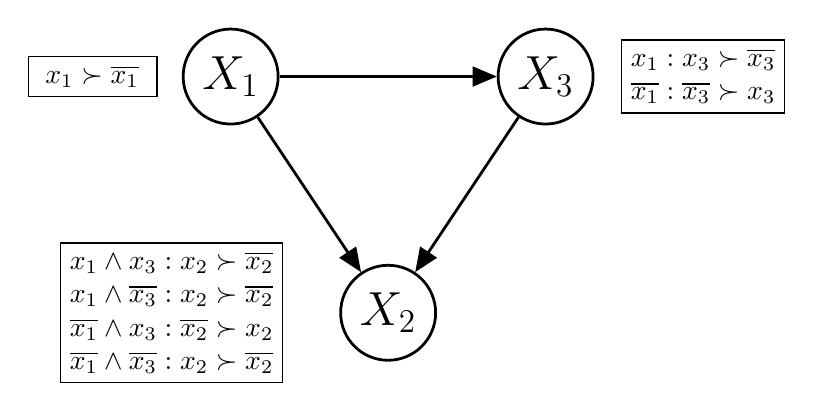
\begin{tikzpicture}[scale=1.0,line width=1.00pt]
      \node [draw,circle,align=center,minimum size=2.75em] (2) at (2, 0) {\LARGE $X_2$};
      \node [draw,circle,align=center,minimum size=2.75em] (1) at (0, 3) {\LARGE $X_1$};
      \node [draw,circle,align=center,minimum size=2.75em] (3) at (4, 3) {\LARGE $X_3$};
      
      \draw [-triangle 45]  (1) -- (3);
      \draw [-triangle 45]  (1) -- (2);
      \draw [-triangle 45]  (3) -- (2);
      
      \node [draw,rectangle,align=center,line width=0.6pt] (c2) at (-0.75,0) {%
        $x_1\land x_3 : x_2\succ \overline{x_2}$\\
        $x_1\land \overline{x_3} : x_2\succ \overline{x_2}$\\
        $\overline{x_1}\land x_3 : \overline{x_2}\succ x_2$\\
        $\overline{x_1}\land\overline{x_3} : x_2\succ \overline{x_2}$
      };
      \node [draw,rectangle,align=center,line width=0.6pt] (c3) at (-1.75,3) {%
        $\;x_1\succ \overline{x_1}$
      };
      \node [draw,rectangle,align=center,line width=0.6pt] (c1) at (6.0,3) {%
        $x_1 : x_3\succ \overline{x_3}$\\
        $\overline{x_1} : \overline{x_3} \succ x_3$
      };
    \end{tikzpicture}
  }
  % \includegraphics[width=0.60\linewidth]{graphics/degenCPnet-eps-converted-to.pdf}
\end{center}
  
\subsection{The \texttt{-d} parameter: a two-node multi-valued example}

It is possible to generate CP-nets with multivalued domains with the
\texttt{-d} option.  Note that our method assumes domain sizes are
\emph{homogeneous}, that is, the same for all variables.  For example,
we can generate an example with 2 nodes ($n=2$) and three-valued
domains ($d=3$) with:
%%
\begin{verbnobox}[\tiny\arabic{VerbboxLineNo}\small\hspace{3ex}]
$ ./gencpnet -n 2 -d 3 examples
Building distribution tables for CP-nets with the following specs:
Number of nodes: n = 2
Bound on in-degree c = 1
Homogeneous domains of size d = 3
Probability of incompleteness i = 0
Generating 1 random CP-nets with these specs.
Generation complete.
$ cat examples/cpnet_n2c1d3_0000.xml
<PREFERENCE-SPECIFICATION>

<PREFERENCE-VARIABLE>
 <VARIABLE-NAME>x1</VARIABLE-NAME>
 <DOMAIN-VALUE>1</DOMAIN-VALUE>
 <DOMAIN-VALUE>2</DOMAIN-VALUE>
 <DOMAIN-VALUE>3</DOMAIN-VALUE>
</PREFERENCE-VARIABLE>

<PREFERENCE-VARIABLE>
 <VARIABLE-NAME>x2</VARIABLE-NAME>
 <DOMAIN-VALUE>1</DOMAIN-VALUE>
 <DOMAIN-VALUE>2</DOMAIN-VALUE>
 <DOMAIN-VALUE>3</DOMAIN-VALUE>
</PREFERENCE-VARIABLE>

<PREFERENCE-STATEMENT>
  <STATEMENT-ID>p1_1</STATEMENT-ID>
  <PREFERENCE-VARIABLE>x1</PREFERENCE-VARIABLE>
  <PREFERENCE>2:1</PREFERENCE>
  <PREFERENCE>1:3</PREFERENCE>
</PREFERENCE-STATEMENT>

<PREFERENCE-STATEMENT>
  <STATEMENT-ID>p2_1</STATEMENT-ID>
  <PREFERENCE-VARIABLE>x2</PREFERENCE-VARIABLE>
  <CONDITION>x1=1</CONDITION>
  <PREFERENCE>2:1</PREFERENCE>
  <PREFERENCE>1:3</PREFERENCE>
</PREFERENCE-STATEMENT>

<PREFERENCE-STATEMENT>
  <STATEMENT-ID>p2_2</STATEMENT-ID>
  <PREFERENCE-VARIABLE>x2</PREFERENCE-VARIABLE>
  <CONDITION>x1=2</CONDITION>
  <PREFERENCE>1:2</PREFERENCE>
  <PREFERENCE>2:3</PREFERENCE>
</PREFERENCE-STATEMENT>

<PREFERENCE-STATEMENT>
  <STATEMENT-ID>p2_3</STATEMENT-ID>
  <PREFERENCE-VARIABLE>x2</PREFERENCE-VARIABLE>
  <CONDITION>x1=3</CONDITION>
  <PREFERENCE>3:1</PREFERENCE>
  <PREFERENCE>1:2</PREFERENCE>
</PREFERENCE-STATEMENT>

</PREFERENCE-SPECIFICATION>
\end{verbnobox}

Again, each generated instance is random and thus probably differs
from what is shown above.  This time the \texttt{PREFERENCE-VARIABLE}
enclosures show that there are two variables, $X_1$ and $X_2$, each
with \emph{three} values, 1, 2, and 3.  We can write these as
$\dom(X_1) = \{x_1, x_1', x_1''\}$, etc.
%%
The first \texttt{PREFERENCE-STATEMENT} enclosure in lines 26--31
tells us that the preference over $X_1$ is unconditional, with
$x_1' \succ x_1 \succ x_1''$.
%%
The following three preference statements (rules) in lines 33--55 give
the CPT for $X_2$.  Note that there is one rule for each assignment to
$X_1$, the parent of $X_2$.  Thus the corresponding CP-net is:

\begin{center}
  \scalebox{0.90}{
    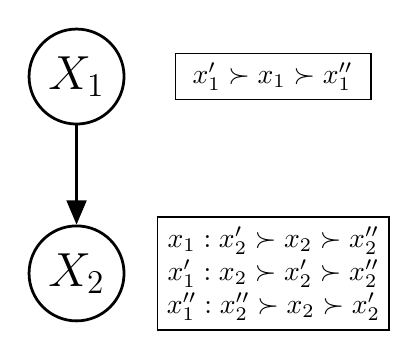
\begin{tikzpicture}[scale=1.0,line width=1.00pt]
      \node [draw,circle,align=center,minimum size=2.75em] (1) at (0, 2.5) {\LARGE $X_1$};
      \node [draw,circle,align=center,minimum size=2.75em] (2) at (0, 0) {\LARGE $X_2$};
      
      \draw [-triangle 45]  (1) -- (2);
      
      \node [draw,rectangle,align=center,line width=0.6pt] (c1) at (2.5,2.5) {%
        $\;x_1'\succ x_1 \succ x_1''$
      };
      \node [draw,rectangle,align=center,line width=0.6pt] (c2) at (2.5,0) {%
        $x_1 : x_2'\succ x_2\succ x_2''$\\
        $x_1' : x_2\succ x_2'\succ x_2''$\\
        $x_1'' : x_2''\succ x_2\succ x_2'$
      };
    \end{tikzpicture}
  }
  % \includegraphics[width=0.60\linewidth]{graphics/degenCPnet-eps-converted-to.pdf}
\end{center}

\subsection{The \texttt{-c} and \texttt{-g} parameters: multiple CP-nets with bounded indegree}

Usually we want to generate a set of CP-nets for an experiment.
We can specify the size of the set with the \texttt{-g} parameter. 
Also, a bound on indegree is customarily assumed; we can specify this
bound with the \texttt{-c} parameter.

Suppose we want to generate 10 CP-nets uniformly at random.  The
CP-nets should have 10 nodes.  No node should have more than 4
parents.  The domains are binary.  We can do this by typing:
%%
\begin{verbatim}
$ ./gencpnet -n 10 -c 4 -d 2 -g 10 temp
Building distribution tables for CP-nets with the following specs:
Number of nodes: n = 10
Bound on in-degree c = 4
Homogeneous domains of size d = 2
Probability of incompleteness i = 0
Generating 10 random CP-nets with these specs.
Generation complete.
\end{verbatim}
%%
The options 
\texttt{-n}, 
\texttt{-c}, 
and \texttt{-d}, 
specify the number of nodes $n$, bound $c$ on indegree, and the size
$d$ of all domains, as described in our paper.  The \texttt{-g} option 
specifies the number of CP-nets to generate.  In this case the
resulting CP-nets are written to the \texttt{temp} subdirectory, which
we can create using \texttt{mkdir} as shown above.
%%
Note that if we had failed to create the new subdirectory, we would
receive an error message:
\begin{verbatim}
Error: cannot open output file cpnet_n10c4d2_0000.xml
Make sure specified directory temp is accessible.
\end{verbatim}
%%
The files are named \verb|cpnet_n10c4d2_0000.xml|,
\verb|cpnet_n10c4d2_0001.xml|, etc.  The numbers after the \texttt{n},
\texttt{c}, and \texttt{d} correspond respectively to the number of
nodes, bound on indegree, and homogeneous domain size as described
above.  The numerals \texttt{0000}, \texttt{0001}, \ldots,
\texttt{0009} index the generated instances.

If the \texttt{-c} parameter is omitted, GenCPnet assumes a default
value of 5.  It is possible to generate CP-nets with unbounded
indegree by specifying a ``bound'' of $c = n-1$, 
%% 
or by specifying an ``infinite'' bound, i.e., \texttt{-c 99}, in which
case the program sets $c$ to $n-1$ internally.  For example,
%%
\begin{verbatim}
./gencpnet -n 20 -c 19 temp
\end{verbatim}
%%
generates just one CP-net with binary valued domains, $n=20$ nodes,
and indegree that is effectively unbounded.  However, with high
probability, the resulting CP-net will have one node with indegree 19,
resulting in a conditional preference table with $2^{19} = 524288$
entries.  The resulting file will be nearly 1~GB in size.  If the
tables are considerably larger even than this, it may be impossible to
output the resulting CP-net representation.  For example:
%%
\begin{verbnobox}[\small]
$ ./gencpnet -n 60 -c 59 temp
Building distribution tables for CP-nets with the following specs:
Number of nodes: n = 60
Bound on in-degree c = 59
Homogeneous domains of size d = 2
Probability of incompleteness i = 0
Sorry, there is not enough memory for CPTs with 576460752303423488 (5.76461e+17) entries
Aborting generation.
\end{verbnobox}
%% 
A suitable bound on indegree is thus conventionally assumed.  For example,
the command 
\begin{verbatim}
./gencpnet -n 60 -c 5 -g 100 temp
\end{verbatim}
%%
should complete in approximately 10--15 seconds, producing 100 files,
each around 270~KB in size.

Note that presently the number of nodes is limited to $n=63$.
An error message will result for $n\ge 64$.  This is a due to our
implementation, which assumes a processor with 64-bit words.  

\subsection{Generating DT problems with \texttt{-t} and \texttt{-h}}

Dominance Testing (DT), determining whether one outcome is preferred
to another, is an important reasoning problem when working with
CP-nets.  With GenCPnet the \texttt{-t} option can be used to generate
\emph{DT problem instances}, as well as CP-net instances, that are
quiprobable with respect to a set of DT problems parameterized by the
number of nodes $n$, bound $c$ on indegree, and homogeneous domain
size $d$.  It is also possible to constrain the Hamming distance, $h$,
of the resulting problem set---that is, to fix the number of variables
in which each outcome pair differs.  

For example, the following generates 10 random CP-nets with 5 nodes,
bound 2 on indegree, and binary domains.  
\begin{verbatim}
./gencpnet -n 5 -c 2 -g 10 -t 1 problems
\end{verbatim}
For each CP-net, one pair of
outcomes (unconstrained by Hamming distance) is also generated. 
A listing of the directory gives:
\begin{verbnobox}[\small]
-rw-rw-r-- 1 user user 4006 Dec 10 17:01 cpnet_n5c2d2_0000.xml
-rw-rw-r-- 1 user user 3783 Dec 10 17:01 cpnet_n5c2d2_0001.xml
-rw-rw-r-- 1 user user 4006 Dec 10 17:01 cpnet_n5c2d2_0002.xml
-rw-rw-r-- 1 user user 4006 Dec 10 17:01 cpnet_n5c2d2_0003.xml
-rw-rw-r-- 1 user user 4006 Dec 10 17:01 cpnet_n5c2d2_0004.xml
-rw-rw-r-- 1 user user 3783 Dec 10 17:01 cpnet_n5c2d2_0005.xml
-rw-rw-r-- 1 user user 3277 Dec 10 17:01 cpnet_n5c2d2_0006.xml
-rw-rw-r-- 1 user user 3500 Dec 10 17:01 cpnet_n5c2d2_0007.xml
-rw-rw-r-- 1 user user 3500 Dec 10 17:01 cpnet_n5c2d2_0008.xml
-rw-rw-r-- 1 user user 4006 Dec 10 17:01 cpnet_n5c2d2_0009.xml
-rw-rw-r-- 1 user user 1452 Dec 10 17:01 dt_n5c2d2_0000_0000.xml
-rw-rw-r-- 1 user user 1452 Dec 10 17:01 dt_n5c2d2_0001_0000.xml
-rw-rw-r-- 1 user user 1452 Dec 10 17:01 dt_n5c2d2_0002_0000.xml
-rw-rw-r-- 1 user user 1452 Dec 10 17:01 dt_n5c2d2_0003_0000.xml
-rw-rw-r-- 1 user user 1452 Dec 10 17:01 dt_n5c2d2_0004_0000.xml
-rw-rw-r-- 1 user user 1452 Dec 10 17:01 dt_n5c2d2_0005_0000.xml
-rw-rw-r-- 1 user user 1452 Dec 10 17:01 dt_n5c2d2_0006_0000.xml
-rw-rw-r-- 1 user user 1452 Dec 10 17:01 dt_n5c2d2_0007_0000.xml
-rw-rw-r-- 1 user user 1452 Dec 10 17:01 dt_n5c2d2_0008_0000.xml
-rw-rw-r-- 1 user user 1452 Dec 10 17:01 dt_n5c2d2_0009_0000.xml
\end{verbnobox}
Here the XML files prefaced with \verb|cpnet_| describe CP-nets as
explained above.  Those prefaced with \verb|dt_| describe DT problem
instances.  Note that the filename for each DT instance contains
\emph{two} indices.  The first is the same as the index of the
corresponding CP-net.  The second is numbered sequentially from 0000.
If we had generated multiple DT problems for CP-net 0000, then the
corresponding DT XML files would be labeled \verb|0000_0000|,
\verb|0000_0001|, etc.

Recall that a DT problem $\mathcal{N} \models o \succ o'$ consists of
a CP-net $\mathcal{N}$ and a pair of outcomes $o$ and $o'$.  It is
assumed, of course, that $\mathcal{N}$, $o$, and $o'$ share the same
set of variables $\mathcal{V}$ with associated domains.  
%%
Consider the randomly generated contents of \verb|dt_n5c2d2_0000_0000.xml|:
%%
\begin{verbnobox}[\tiny\arabic{VerbboxLineNo}\small\hspace{3ex}]
<PREFERENCE-QUERY>
  <PREFERENCE-SPECIFICATION-FILENAME>cpnet_n5c2d2_0000.xml</PREFERENCE-SPECIFICATION-FILENAME>
  <QUERY-TYPE>DOMINANCE</QUERY-TYPE>
  <OUTCOME>
    <LABEL>BETTER</LABEL>
    <ASSIGNMENT>
      <PREFERENCE-VARIABLE>x1</PREFERENCE-VARIABLE>
      <VALUATION>2</VALUATION>
    </ASSIGNMENT>
    <ASSIGNMENT>
      <PREFERENCE-VARIABLE>x2</PREFERENCE-VARIABLE>
      <VALUATION>1</VALUATION>
    </ASSIGNMENT>
    <ASSIGNMENT>
      <PREFERENCE-VARIABLE>x3</PREFERENCE-VARIABLE>
      <VALUATION>2</VALUATION>
    </ASSIGNMENT>
    <ASSIGNMENT>
      <PREFERENCE-VARIABLE>x4</PREFERENCE-VARIABLE>
      <VALUATION>2</VALUATION>
    </ASSIGNMENT>
    <ASSIGNMENT>
      <PREFERENCE-VARIABLE>x5</PREFERENCE-VARIABLE>
      <VALUATION>2</VALUATION>
    </ASSIGNMENT>
  </OUTCOME>
  <OUTCOME>
    <LABEL>WORSE</LABEL>
    <ASSIGNMENT>
      <PREFERENCE-VARIABLE>x1</PREFERENCE-VARIABLE>
      <VALUATION>2</VALUATION>
    </ASSIGNMENT>
    <ASSIGNMENT>
      <PREFERENCE-VARIABLE>x2</PREFERENCE-VARIABLE>
      <VALUATION>2</VALUATION>
    </ASSIGNMENT>
    <ASSIGNMENT>
      <PREFERENCE-VARIABLE>x3</PREFERENCE-VARIABLE>
      <VALUATION>2</VALUATION>
    </ASSIGNMENT>
    <ASSIGNMENT>
      <PREFERENCE-VARIABLE>x4</PREFERENCE-VARIABLE>
      <VALUATION>1</VALUATION>
    </ASSIGNMENT>
    <ASSIGNMENT>
      <PREFERENCE-VARIABLE>x5</PREFERENCE-VARIABLE>
      <VALUATION>1</VALUATION>
    </ASSIGNMENT>
  </OUTCOME>
</PREFERENCE-QUERY>
\end{verbnobox}
%%
The \verb|PREFERENCE-SPECIFICATION-FILENAME| enclosure gives the XML
file specifying CP-net $\mathcal{N}$.  The two \verb|outcome|
enclosures specify the outcomes $o$ and $o'$.  In this case, the
problem is whether
$ \overline{x_1}\,x_2\,\overline{x_3}\,\overline{x_4}\,\overline{x_5}
\succ \overline{x_1}\,\overline{x_2}\,\overline{x_3}\,x_4\,x_5$
with respect to CP-net $\mathcal{N}$ as defined in the file
\verb|cpnet_n5c2d2_0000.xml|.
%%
Again, we refer the reader to the page
\url{http://www.ece.iastate.edu/~gsanthan/crisner.html} for additional
details on the XML specification.

Note that in the problem given above, the Hamming distance is 3, since
the two values differ in the values of $X_2$, $X_4$, and $X_5$.  We
could constrain the Hamming distance to any given value between 1 and
$n$ inclusive with the \verb|-h| option.  For example:

\begin{verbatim}
./gencpnet -n 5 -c 2 -g 10 -t 1 -h 2 problems
\end{verbatim}

We can use \verb|-t 10| to generate 10 DT problems for each of 10
CP-nets---a total of 100 DT problems:
\begin{verbatim}
./gencpnet -n 20 -c 4 -g 10 -t 10 problems
\end{verbatim}

\subsection{Other command line parameters}

The \texttt{--quiet} parameter can be used to silence all most of the
output to the console.  Conversely, \texttt{--verbose} provides
additional output for debugging purposes. 

An experimental \texttt{-i} parameter allows specifying a \emph{degree
  of incompleteness}.  For example, \texttt{-i 0.60} specifies that
each conditional preference rule will be specified with probability
0.6.  Note that this does not mean that \emph{exactly} 60\% of the
rules of each table will be filled; it is only a probability invoked
for each rule.  Thus the actual generated table could be complete or
empty.  \textbf{This is an experimental feature.  As such, it could be
  removed or its behavior may be modified in a future release.}

Finally, the \texttt{--count} and \texttt{--countdags} parameters only
output the \emph{number} of CP-nets and directed acyclic graphs (DAGs)
respectively, as described in our paper.  For example, the following
BASH shell script
\begin{verbnobox}[\tiny\arabic{VerbboxLineNo}\small\hspace{3ex}]
echo "The number of acyclic, unbounded, binary CP-nets:"
echo -e "n\ta(n)"
for i in $(seq 1 8); do
    echo -n -e $i '\t'
    # Here we use c=9999 as "infinity"; that is, unbounded indegree
    ./gencpnet -n $i -c 9999 -d 2 --count --quiet .
    echo
done
\end{verbnobox}
produces the output:
\begin{verbnobox}[\small]
The number of acyclic, unbounded, binary CP-nets:
n    a(n)
1    2
2    12
3    488
4    481776
5    157549032992
6    4059976627283664056256
7    524253448460177960474729517490503566696576
8    1427153634467948627654814418603596566233315529747076624457951655059580698906328832
\end{verbnobox}
%%
Note also the use of the \texttt{--quiet} option.
The complete script is included in the distribution as \texttt{count.sh}. 

\section{License}

GenCPnet is free software,
released under the GNU Public License version 3.
You should have received a copy of \texttt{gpl-3.0.txt} in the
archive.  If not, see \url{http://www.gnu.org/licenses/}.

If you use GenCPnet in your research, we hope you will choose to
cite our paper.  \BibTeX{} format is:
\begin{verbnobox}[\small]
@inproceedings{generating_cpnets,
  title  = {Generating {CP}-nets Uniformly at Random},
  author = {Thomas E. Allen and 
    Judy Goldsmith and Hayden Elizabeth Justice and Nicholas Mattei and Kayla Raines},
  booktitle={Procedings of the 30th AAAI Conference on Artificial Intelligence (AAAI-16)},
  note = {To appear},
  year = {2016}
}
\end{verbnobox}

\bibliography{Gencpnet_guide}
\bibliographystyle{plain}

\end{document}
